As mentioned, two of the samples are MBD2 IPs, and two are inputs. Therefore, the IP samples should differ to the inputs in at least two ways. Firstly, they should be more CpG-rich, since we are enriching for methylated DNA, whcih rarely occurs outside of this sequence context. Secondly, DNA methylation tends to occur in peaks since CpG sites are often present in CpG-rich islands.  Conversely, the input samples should be distributed somewhat uniform genome-wide, aside from the usual mappability and GC content biases.\\

We can visualize the (log) frequencies of normalized coverage to get an idea of whether the reads occur in clusters or more dispersed, at least in a relative sense.  For this, we can use \texttt{enrichmentPlot}.  Similarly, we can calculate the CpG density of reads (or reads extended to a certain fragment size) and plot distributions across multiple samples using \texttt{cpgDensityPlot}, as below.

\begin{Schunk}
\begin{Sinput}
 seqinfo(samples.list)
\end{Sinput}
\begin{Soutput}
Seqinfo of length 25
seqnames seqlengths isCircular
chr1      247249719       <NA>
chr2      242951149       <NA>
chr3      199501827       <NA>
chr4      191273063       <NA>
chr5      180857866       <NA>
chr6      170899992       <NA>
chr7      158821424       <NA>
chr8      146274826       <NA>
chr9      140273252       <NA>
...             ...        ...
chr17      78774742       <NA>
chr18      76117153       <NA>
chr19      63811651       <NA>
chr20      62435964       <NA>
chr21      46944323       <NA>
chr22      49691432       <NA>
chrX      154913754       <NA>
chrY       57772954       <NA>
chrM          16571       <NA>
\end{Soutput}
\begin{Sinput}
 enrichmentPlot(samples.list, seq.len = 300, cols = c("black", 
     "green", "orange", "red"), xlim = c(0, 10), lwd = 2)
\end{Sinput}
\end{Schunk}
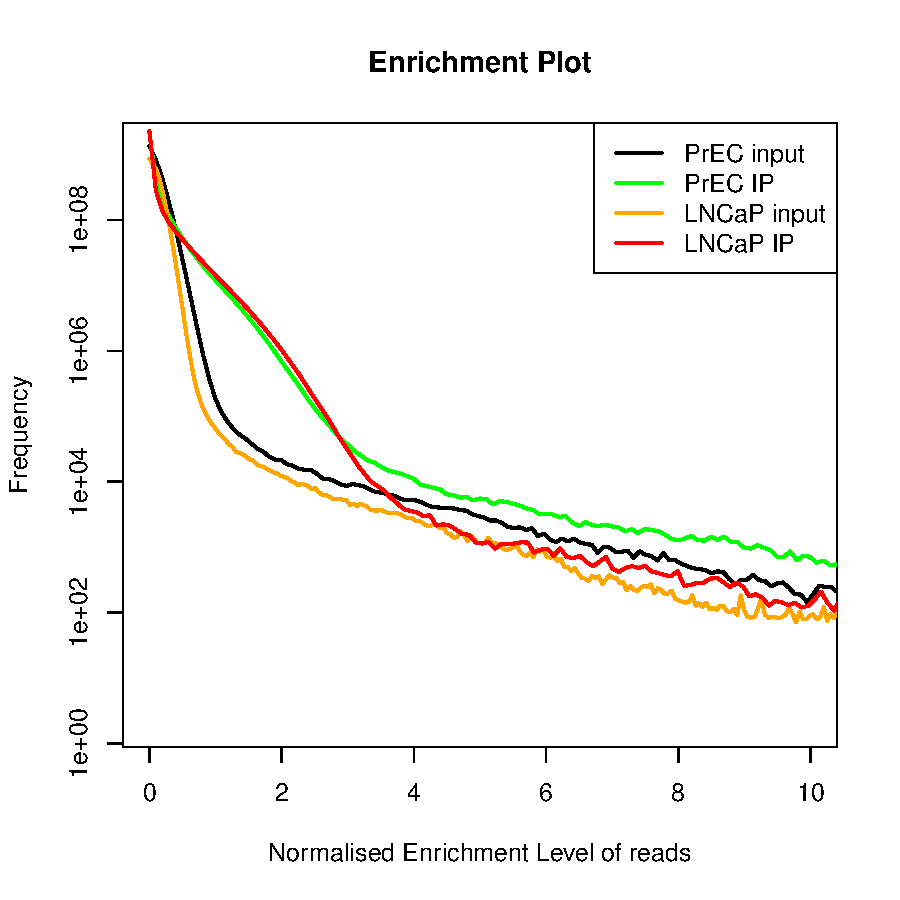
\includegraphics{qc-enrPlot}

\noindent The code makes use of the SeqInfo annotation of \texttt{samples.list} to retrieve the maximum base of chromosomes.  Normalization scales coverage value to ``reads per 10 million". The argument \texttt{seq.len=300} is passed in as the length to extend reads to, since that is approximately the real length of the fragments sequenced in this experiment. As expected, many more bases in the IP samples have high read coverages. \\
\ \\
An alternative comparative visualization, which is somewhat specific to methylated DNA enrichment experiments, is a summary of the distribution of CpG density among reads/fragments:

\begin{Schunk}
\begin{Sinput}
 library(BSgenome.Hsapiens.UCSC.hg18)
 cpgDensityPlot(samples.list, organism = Hsapiens, w.function = "none", 
     seq.len = 300, cols = c("black", "green", "orange", "red"), 
     xlim = c(0, 30), lwd = 2)
\end{Sinput}
\end{Schunk}
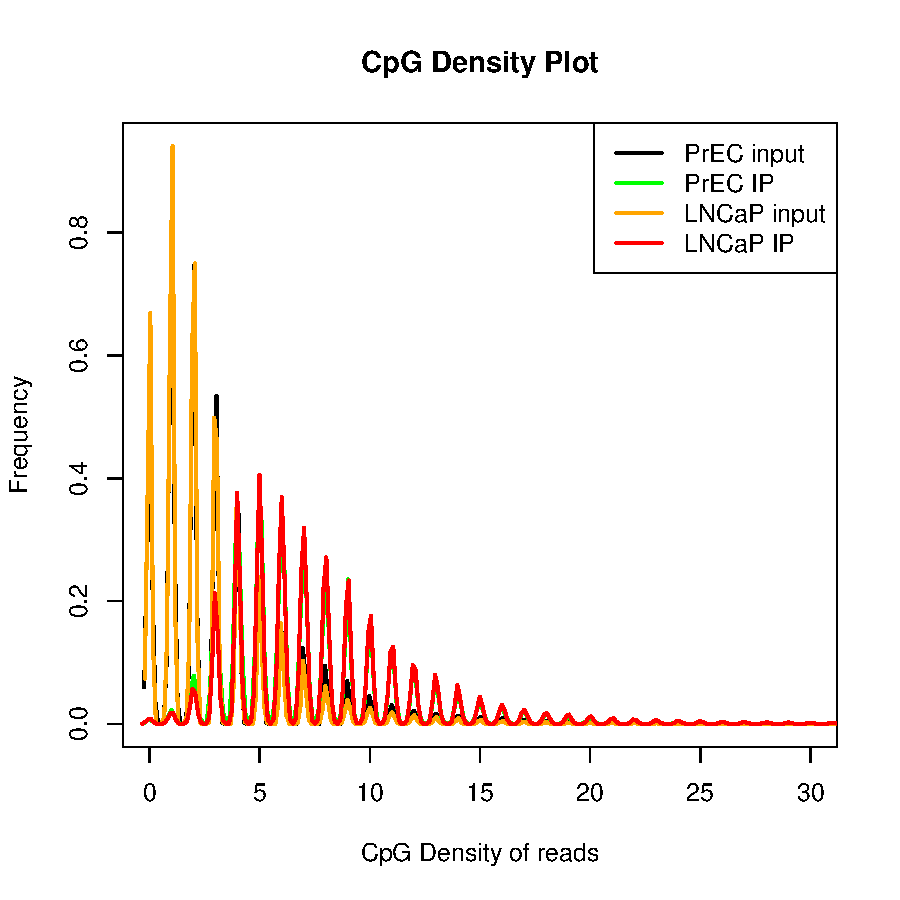
\includegraphics{qc-cpgPlot}

\noindent The full genome sequence of the organism is required so that the (here, 300 base) DNA sequence can be fetched. In this example, the \texttt{BSgenome} package of the hg18 assembly for human is used (many other BSgenome objects for other organisms are available from Bioconductor). The \texttt{w.function} parameter allows the count of CpGs to be weighted. In this example, raw counts are used.
\ \\ \ \\
Notice that at lower CpG densities, the two input samples have a higher frequency of reads than the two IP samples. At higher CpG densities, this trend is reversed. This suggests that the enrichment of methylated CpGs has worked.
\ \\ \ \\
% \noindent For more general sequencing quality checking, the FastQC \footnote{\href{http://www.bioinformatics.bbsrc.ac.uk/projects/fastqc/}{http://www.bioinformatics.bbsrc.ac.uk/projects/fastqc/}} Java application has been gaining popularity due to its speed and variety of results. A container class, \texttt{FastQC}, accessors, and the method \texttt{readFastQC} for reading in the raw Java program text file output and creating a FastQC \textbf{R} object, have been made to provide a framework for the fast development of quality control report generating pipelines. Higher level container classes with accessor methods are \texttt{SequenceQC}, which groups \texttt{FastQC} objects for the aligned and unaligned reads of a single sample together, and \texttt{SequenceQCSet} which is a collection of \texttt{SequenceQC} objects, perhaps of multiple sequencing samples within the same experimental run.
% \\ \\
% An example of turning a set of FastQC text output files of the DNA methylation read data into a quality report PDF is demonstrated next.

% <<label=QCreport>>=
% load("QCset.RData")
% summary(QCset)

% pdf("QCreport.pdf", height = 8, width = 12)
% genQC(QCset, "DNA Methylation Experiment")
% dev.off()
% @

% Click here to see the report. \attachfile[icon=Paperclip]{QCreport.pdf}
% \\ \\
% When looking at the base distributions of the inputs, for either all of the reads, or the aligned subset, it can be seen that the frequency of A or T is always more than the G or C frequency. This mirrors the background distribution of the human genome. In the IP samples, the G or C frequency has risen, and the A or T has dropped, as would be expected when enriching for GC rich DNA methylated sequences.
% \\ \\
% This mismatches-by-cycles plots show that the IP samples tend to have a bias of G being called as T, and this is independent of the sequencing cycle. PrEC input has a tendency to miscall T as G more often than any other error, no matter the cycle.
